% !TEX root=../main.tex

\chapter{ICARUS-T600 detector operations and event reconstruction}
\label{chap:event_reconstruction}

The ICARUS detector, described in \autoref{sec:ICARUS_T600} is a complex system, and a precise operation is required to make the most out of all its subcomponents. Each part of the online operation is essential and preliminary to the offline operations, consisting of the wireplane signal processing, the reconstruction of all the signals coming from the different subsystems and their combination to obtain a final physics result. 

\section{Data acquisition} \label{sec:DAQ}

The data that comes out of the detector is, much like many other experiments, organised in events. The definition of an event is unique to each experiment, as different experiments collecting different data might prefer one classification  type over another. In the case of LArTPC, an event is defined as the collection of the readout signal from all the wires, each with information on the wire position and orientation, and the raw waveform coming from all the other subdetectors modules --- CRT and PMT --- collected in a time window defined by the properties of each detector starting from a defined $t_0$. Being PMTs a fast technology, the time window of the collected waveforms is smaller than, for example, that of the TPC. The start time $t_0$ is usually defined by means of a triggering system. 

\paragraph{ICARUS trigger} The ICARUS trigger employs the coincidence between the signal from the beams (BNB and NuMI) spill gates with the scintillation light to provide a global signal that activates  the acquisition windows for the TPC and PMT subsystems. For TPC, the acquisition window is driven by the time it takes for drift electrons to cross half of each T300 module: with a nominal electric drift field of \SI{500}{\volt\per\cm}, and a half-width of $\sim\SI{1.5}{\m}$, the drift time is chosen to be $\SI{1.6}{\ms}$. The acquisition window for PMTs is driven by the mean lifetime of LAr excited states. De-excitation of LAr produces scintillation light in two components, one fast $\tau\simeq \SI{6}{\ns}$ and one slow $\tau\simeq\SI{1.6}{\us}$. To collect the full scintillation light, the time window has to be thus greater than \SI{1.6}{\us}. Additionally, in the case of a second light trigger in the \SI{10}{\us} immediate subsequent window --- this could be the case for a cosmic-induced muon crossing the detector during the drifting of the electrons ---, the readout is extended by \SI{7}{\us}. Finally, a \SI{7}{\us} buffer before the global trigger is also kept, adding up to a total of \SI{26}{\us} of PMT acquisition window.  

The ICARUS trigger architecture allows for multiple configurations, i.e. the acquisition of different types of events \cite{ICARUS:2025kai}, with and without beam (on- and off-beam), and requiring or not requiring the PMT light signal (majority or minimum bias). The main ICARUS trigger physics configuration (on-beam majority) is based on the multiplicity of PMT signals in coincidence with the beam ``open'' spill gate. Off-beam cosmic ray events are collected with similar ``off-beam majority'', requiring the coincidence between the light signal and off-beam gates, generated \SI{33}{\ms} after on-beam gates. Minimum bias (both for on- and off-beam configurations) triggers are generated in the presence of the corresponding gate, regardless of the presence of scintillation light.

\paragraph{Collection of the triggered events. } Once a global trigger is present, the data acquisition system (DAQ), which communicates via TCP/IP protocol with the trigger system, activates the readout of the whole detector, with \SI{1.6}{\ms} and \SI{26}{\us} for the TPC and PMTs, respectively. ICARUS DAQ is based on the \emph{artdaq} data acquisition software development kit developed at Fermilab \cite{Biery:2013cda}. The \emph{artdaq} SDK provides  customisable applications for reading data fragments from detector elements, which are identified as \emph{BoardReader} objects in the \emph{artdaq} language, and configurable applications for performing event-building (i.e. merging together the collected data fragments from each \emph{BordReader}, performed by objects inherited from \emph{EventBuilder} instances), data-logging and data-dispatch to downstream online data quality monitoring processes. 

Customised \emph{BoardReaders} acquire data fragments from all ICARUS subdetectors, TPC, PMT and CRT readout electronics, and from trigger and White Rabbit: this latter subsystem, not described in \autoref{sec:ICARUS_T600}, is a CERN-developed technology that provides global timing across all subdetectors and serves also as a double check against trigger global timing. Event counters and timestamps are assigned accordingly to each data fragment, which are then queued for data transfer to a configurable number of \emph{EventBuilder} instances. When an event is triggered, the corresponding trigger \emph{BoardReader} instance sends the trigger data fragment to the \emph{EventBuilder}. This triggers a request for data from all other configured \emph{BoardReader}s in the DAQ system. \autoref{fig:DAQ} shows a simplified illustration of the DAQ working principle. 

\begin{figure}
    \centering
    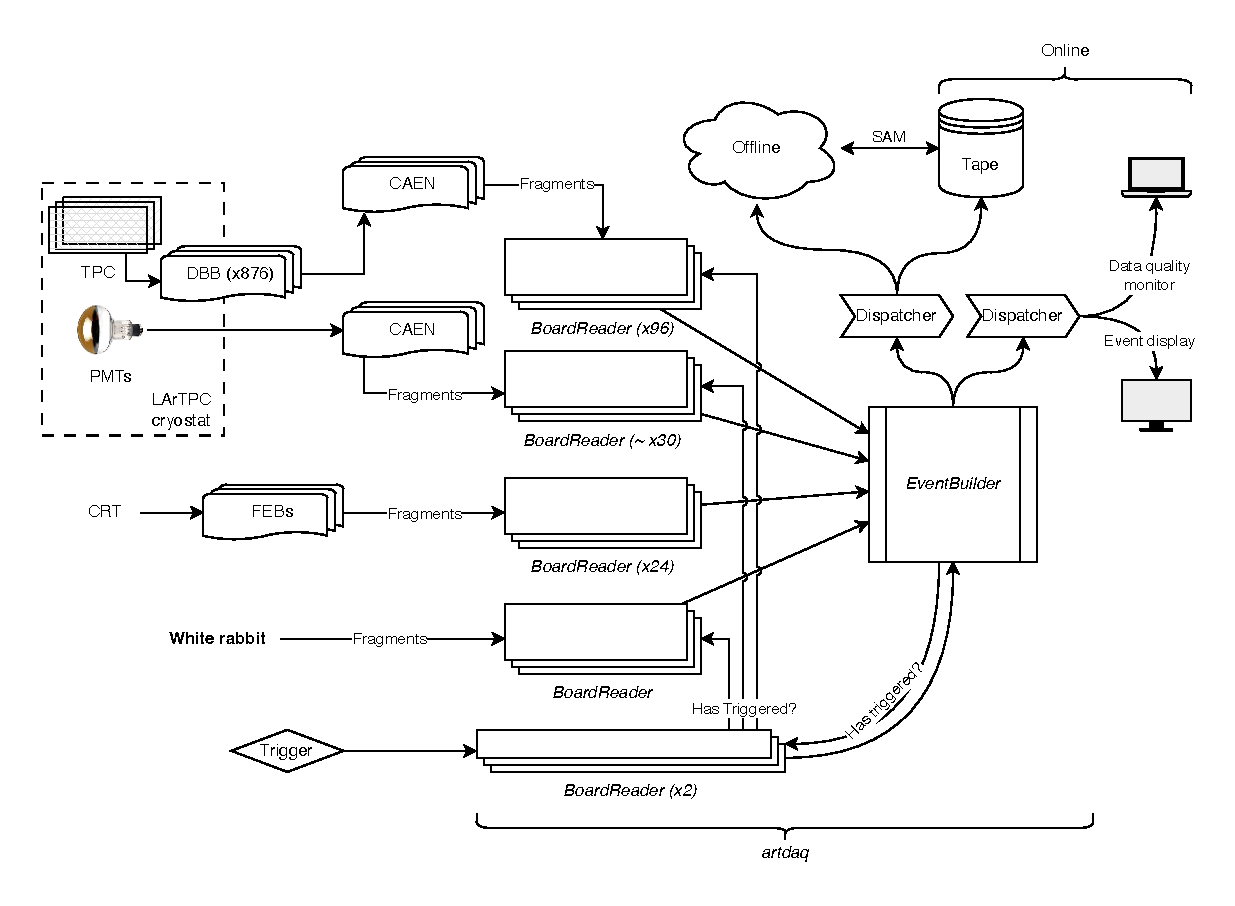
\includegraphics[width=\linewidth]{detector/DAQ_simplified.pdf}
    \caption[ICARUS DAQ illustration]{Simplified illustration of the ICARUS DAQ system. Further information is found in \autoref{sec:DAQ}. The number of parallel \emph{EventBuilder} instances could be defined $\geq1$, to allow for faster processing.}
    \label{fig:DAQ}
\end{figure}

The data collected by the ICARUS DAQ system is written in different file streams depending on which beam it is detecting and which trigger configuration is active, whether on- or off-beam, minimum bias or majority. 

Downstream of the DAQ interface, events are written using the \emph{art} event-processing framework \cite{greenArtFramework2012} also developed at Fermilab, on which the \emph{artdaq} SDK is built. This allows flawless interoperability between the DAQ interface and the offline analysis, without the need to convert the events saved from the DAQ interface into a format compatible with the high-level offline analysis. After a long testing and commissioning phase, the DAQ system was reported to be able to stably handle high data rates up to \SI{5}{\hertz}. This is, however, well in excess of what the detector is supposed to be handling, given the BNB and NuMI data rates when using a majority-based trigger configuration, based on light scintillation, delivering about \SI{1}{\hertz} of data throughput.  

In order to handle the large volumes of data stored on tape, the Fermilab-based SAM (serial access to metadata) system is exploited. This system associates a set of metadata information with each data file using Python scripts. This metadata is useful in offline analysis to create large datasets of files, identifying whether the files contain raw or processed data, run configuration, run number and so on.

\section{ICARUS data processing}

The output data files contain the aggregated data coming from all the \emph{BoardReader} instances in an event. For the TPC, the data correspond to the digitised waveforms from each TPC readout channel, representing the charge induced by the motion of ionisation electrons drifted by the electric field inside the detector. Similarly, the data from the PMTs correspond to the digitised waveforms of the readout of every PMT inside the detector, corresponding of the scintillation light deposited in each PMT. For the CRT system the DAQ process is slightly different \cite{ICARUS:2025rdw,Poppi:2023zmp,Poppi:2022vhg}. The ICARUS CRTs operate in self-trigger mode \cite{arteroponsStudyReconstructionNuMuCC, ICARUS:2025rdw}, whenever a CRT SiPM exceeds the threshold, the data from all 32 SiPM channels for each FEB is stored in internal buffers, holding up to \qtyrange{40}{80}{\ms} depending on which CRT sub-part is considered. The data from the top, bottom and side CRTs is aggregated within \SI{10}{\us} data fragments in the \emph{BoardReader}s instances; once the global trigger is activated, \SI{+-25}{\ms} of CRT data fragments are sent from the \emph{BoardReader} to the \emph{EventBuilder} instance. 

The output of all ICARUS sub-detectors is common across LArTPC detectors, which might have different TPC geometry and light collection configurations but share the same underlying technology. The \emph{art}-based \emph{LArSoft} framework \cite{Church:2013hea,Snider:2017wjd,Pordes:2017BL} is the common software development kit providing software infrastructure and algorithms for simulation of Monte Carlo data, processing of both simulated and real data, and event reconstruction. 

When an event is saved from DAQ to data files and stored to tape, it is then available to be processed. The ICARUS data processing chain is split, like for many other LArTPC detectors, into two \emph{stages}, usually named \emph{Stage0} or \emph{reco1} and \emph{Stage1} or \emph{reco2}. Processing the raw collected data is a mandatory step in order for it to be properly analysed. 

In the \emph{Stage0/reco1} step, all data  from the three sub-detectors is processed to produce a ``simpler'' description of the raw signal. This means to decode the raw signal and translate it into objects in the \emph{LArSoft} format for offline reconstruction. It also performs signal processing of the waveforms to identify physical signals, \emph{Hits}, that can then be used as input to the higher-level event reconstruction tools implemented in the \emph{Stage1/reco2} steps. 

\begin{table}
    \centering
    \begin{tabular}{
    @{}>{\itshape}
    m{0.1\linewidth}
    @{\hspace{0.05\linewidth}}
    p{0.25\linewidth}
    @{\hspace{0.05\linewidth}}
    p{0.25\linewidth}
    @{\hspace{0.05\linewidth}}
    p{0.25\linewidth}
    @{}
    }
         & TPC & PMT & CRT \\
         \hline 
         Stage0 & TPC wire signal decoding & Waveform analysis (pedestrian, thresholds, \dots) & CRT \emph{Hit} finding \\
         & Signal deconvolution & \emph{OpHit} creation & CRT track \\\
         & ROI finding & \emph{OpFlash} creation & \\
         & \emph{Hit} finding & \multicolumn{2}{c}{CRT-PMT matching} \\
         \hline
         Stage1 & \\
    \end{tabular}
    \caption[]{}
    \label{tab:reco_stages}
\end{table}

%% ADD HERE 

\section{Light reconstruction}

One of the first steps in \emph{Stage0} reconstruction addresses the reconstruction of the light signal. Reconstruction of the light signal associated with the event of interest is based on the recorded PMT signals in the events, sampled at \SI{500}{\mega\hertz}. For any event triggered in coincidence with the beam spill, the digitised signals of all 360 PMTs are recorded in \SI{30}{\us} long time intervals. In addition to this data, whenever an off-time cosmic ray event crosses the volume, triggering scintillation light acquired by the PMTs in the \SI{+-1}{\ms} around the beam gate, all 180 PMTs belonging to the T300 module containing the interaction are recorded in \SI{10}{\us} long time intervals. 

The first step in the light reconstruction is the identification of the PMT signal, using a threshold-based approach. To do so, a ``baseline'' has to be defined, which is performed by a sliding window. The pedestal (the \emph{baseline}) is used to then identify the signal over the threshold, using three thresholds defining the start, tail and end points of the PMT hit, called \emph{OpHit}. The algorithm identifies an \emph{OpHit} as the ensemble of these three values and some information about the integral collected charge of the PMT, which is proportional to the light collected. If a start threshold is reached before the end of a previoud \emph{OpHit} the hit is truncated. \autoref{fig:PMT_reco}b shows the example of a PMT with a clear single \emph{OpHit}. 

After individual optical hits are reconstructed, they are clustered together into higher-level objects, called \emph{OpFlash}, corresponding to multiple optical hits happening in proximity inside the detector, hence corresponding to the same physical event inside the volume. \autoref{fig:PMT_reco}a shows multiple PMTs whose \emph{OpHit} are going to be clustered into a single \emph{OpFlash}, corresponding to collected light produced by a single interaction inside the detector. 

All data products created in the \emph{Stage0} PMT processing are saved using the same \emph{LArSoft}-based structure to \emph{ROOT} \cite{rene_brun_2019_3895860} files. 

\begin{figure}
    \centering
    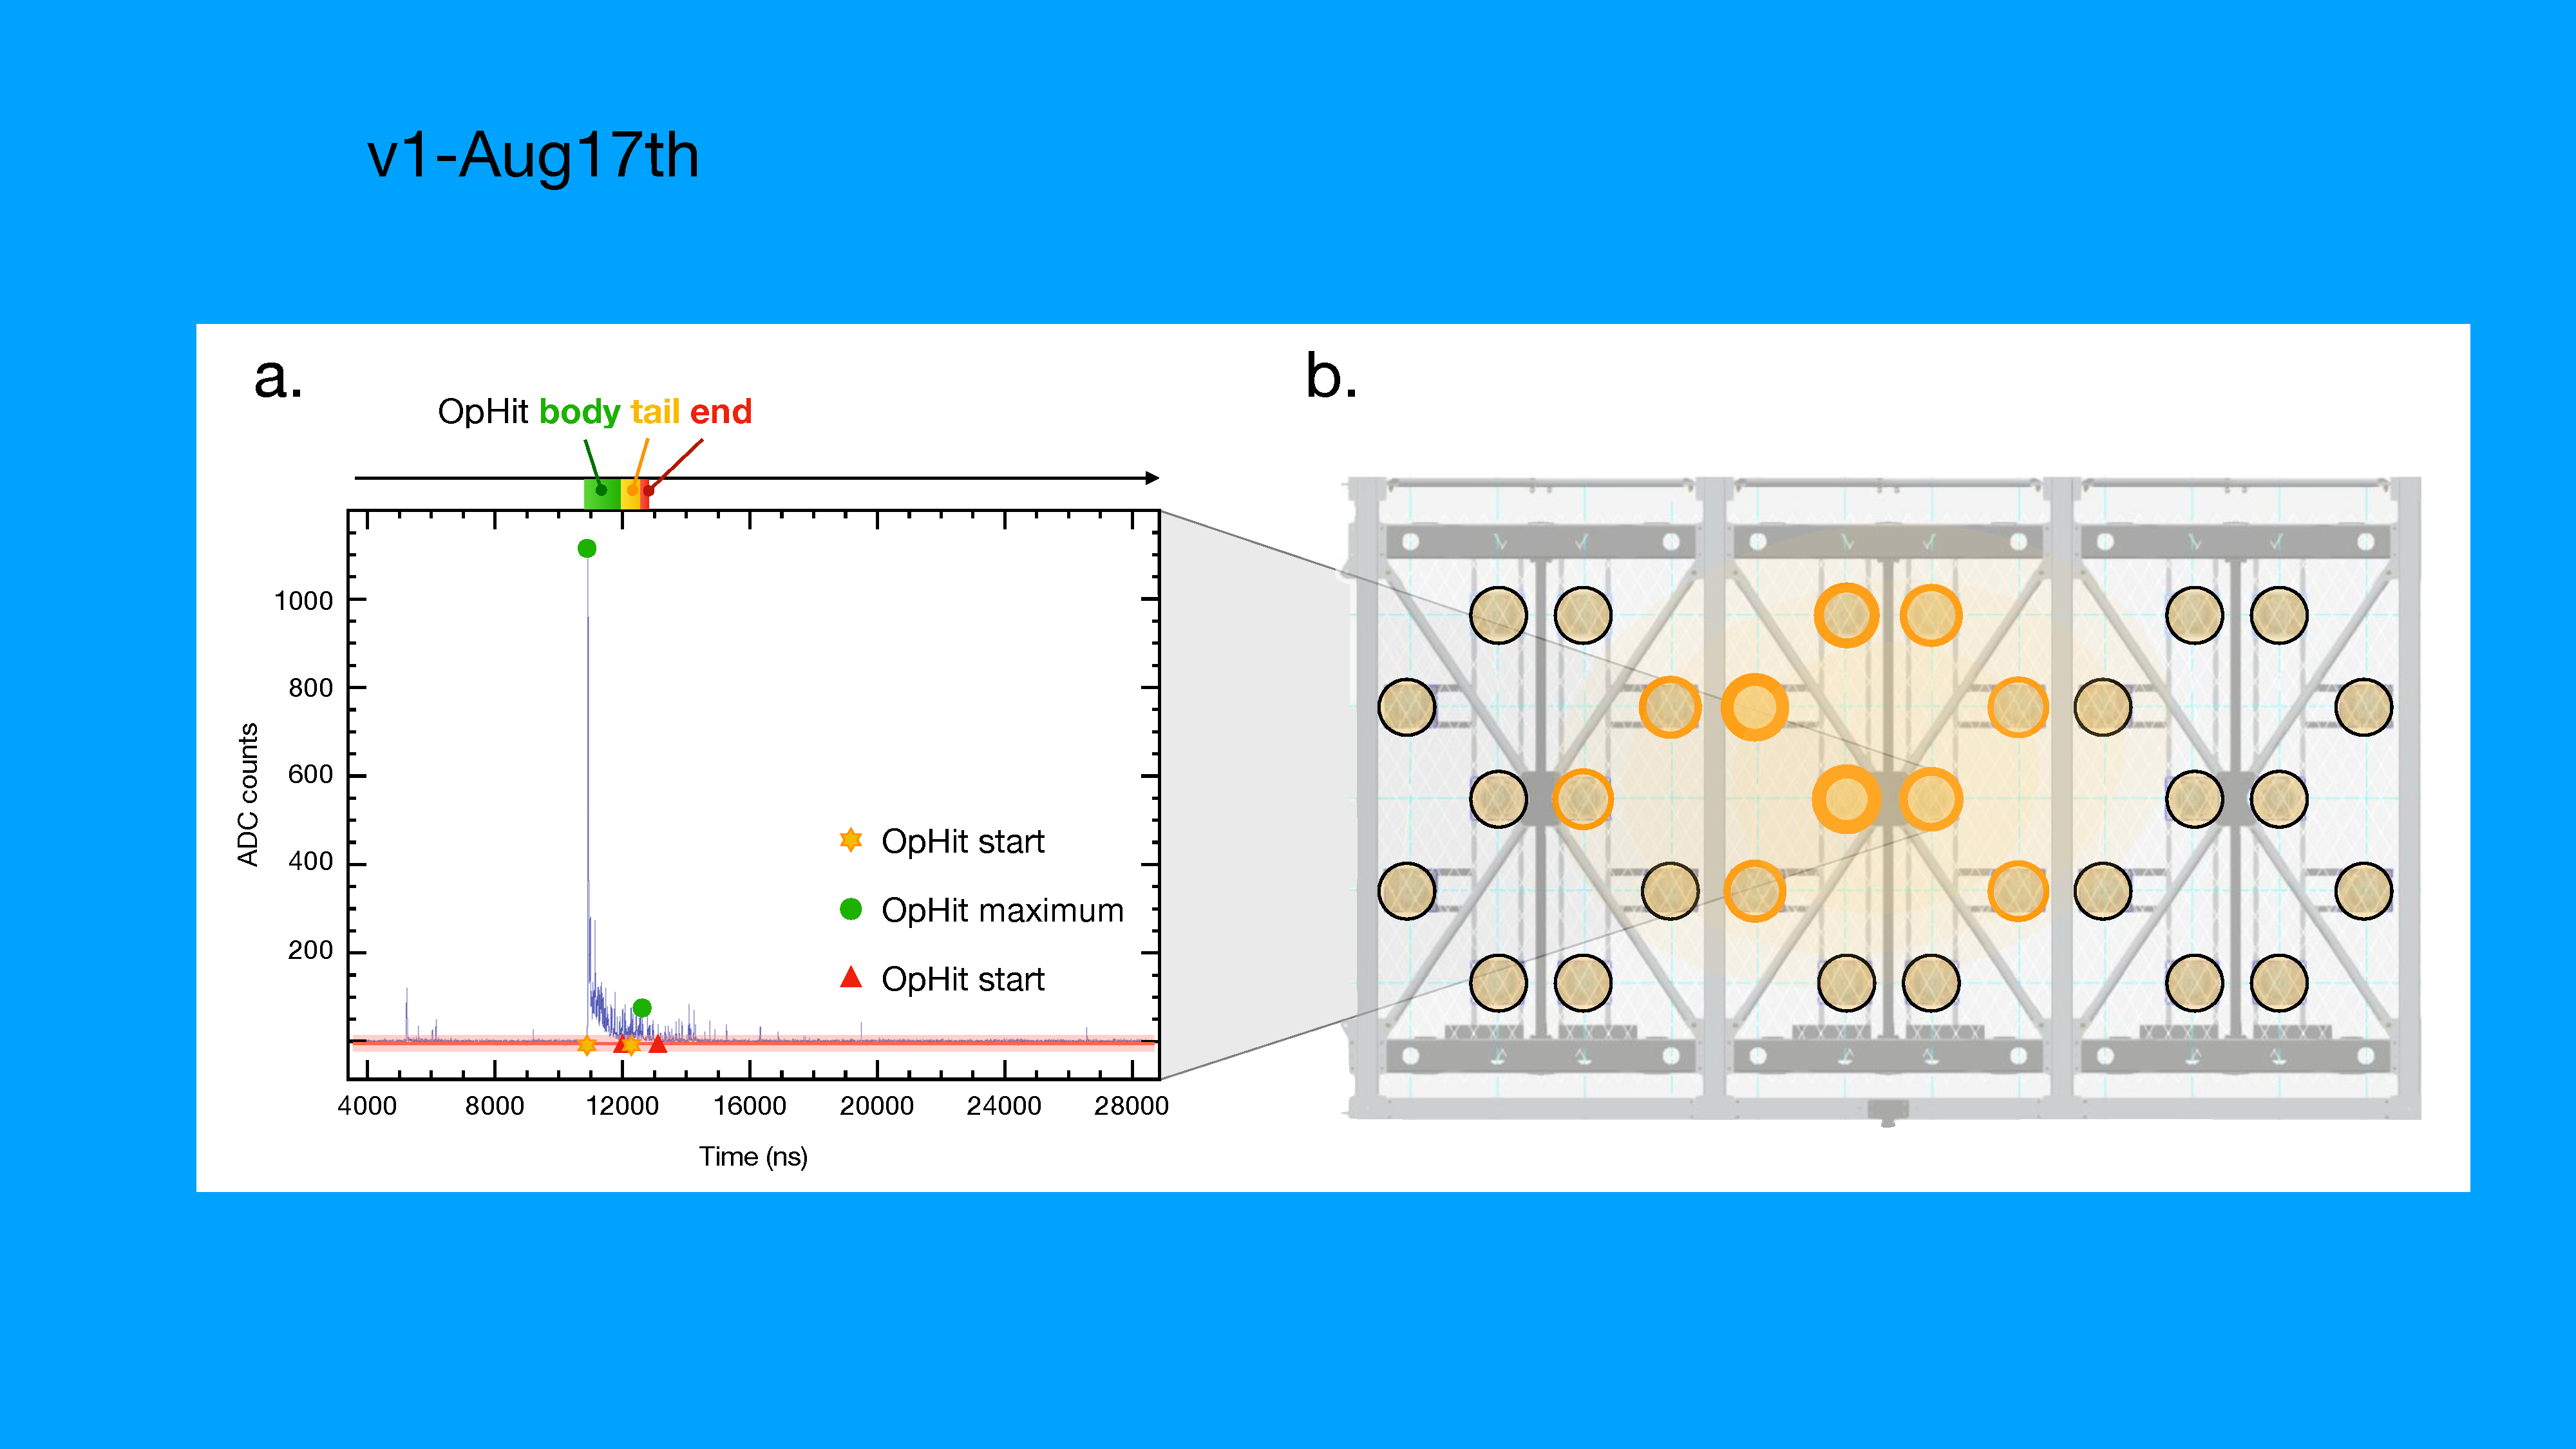
\includegraphics[width=\linewidth,trim={5.5cm 7cm 3.5cm 9cm},clip]{detector/PMT_reco.pdf}
    \caption[PMT reconstructed \emph{OpHits}]{Illustration of an interaction as seen by the PMTs inside the detector volume. (a) shows all the PMTs activated, and a pedestal-subtracted waveform is shown in (b), where also the \emph{OpHit} reconstruction information is pictured. The PMTs which are over threshold in (a), coloured yellow, will constitute the \emph{OpFlash} object.}
    \label{fig:PMT_reco}
\end{figure}

\section{Wireplanes signal reconstruction}

After the PMT data has been processed, it is time for the TPC wire data. The wire data is the waveform readout of the \num{53248} individual wires, with coherent noise removed by the readout cards. Only minimal further processing is performed online, which leaves more scope for reprocessing the raw data using improved signal processing tools. The recorded waveforms are in ADC count/tick units, where the amplitude of the signal is expressed in ADC counts and the time information in ticks, each corresponding to \SI{0.4}{\us} in the ICARUS TPC timing. \autoref{fig:TPC_signal} shows a sample of the data collected by the three planes, exhibiting the characteristic bipolar shape for the two induction wire planes and a unipolar signal for the collection plane. 

\begin{figure}
    \centering
    \subfloat[]{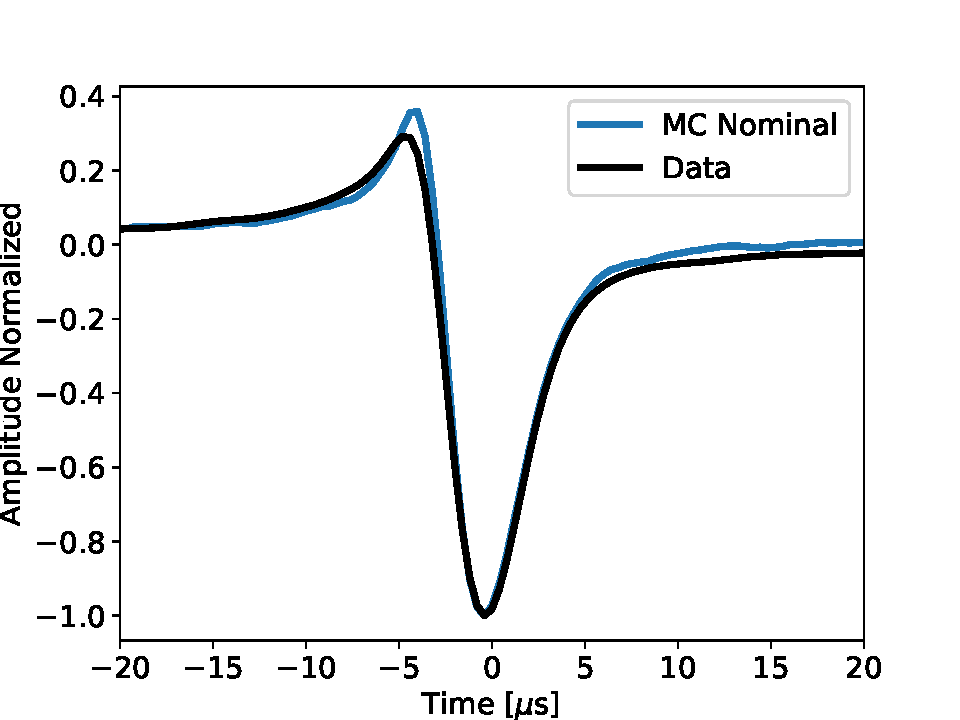
\includegraphics[width=0.3\linewidth]{detector/wvf_data_MCNominal_a20_P0.pdf}\label{fig:TPC_wire_i1}}
    \subfloat[]{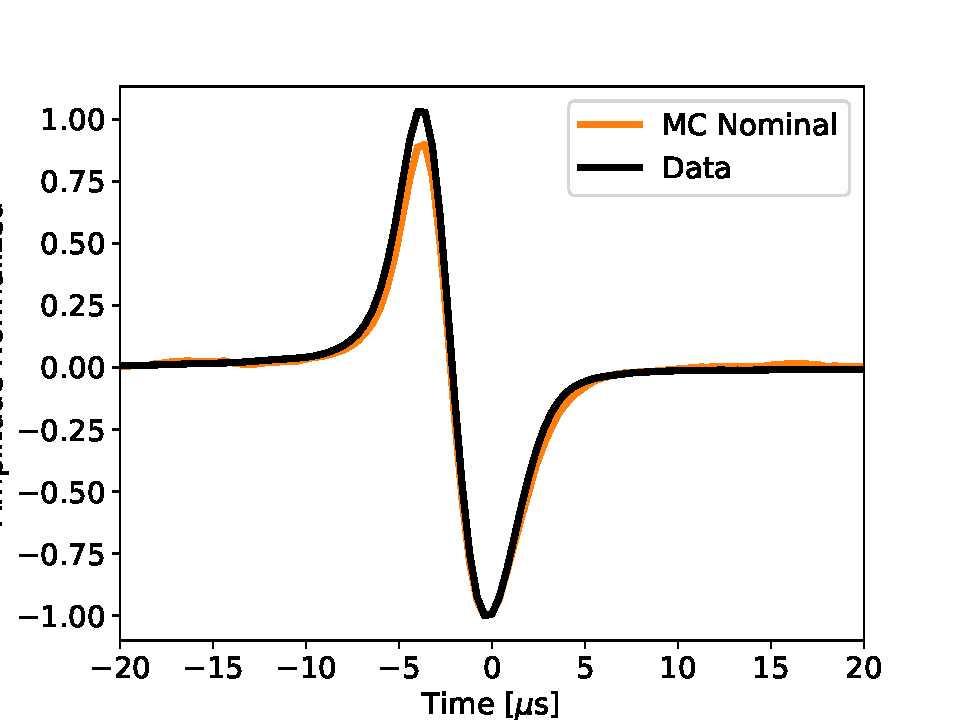
\includegraphics[width=0.3\linewidth]{detector/wvf_data_MCNominal_a20_P1.pdf}\label{fig:TPC_wire_i2}}
    \subfloat[]{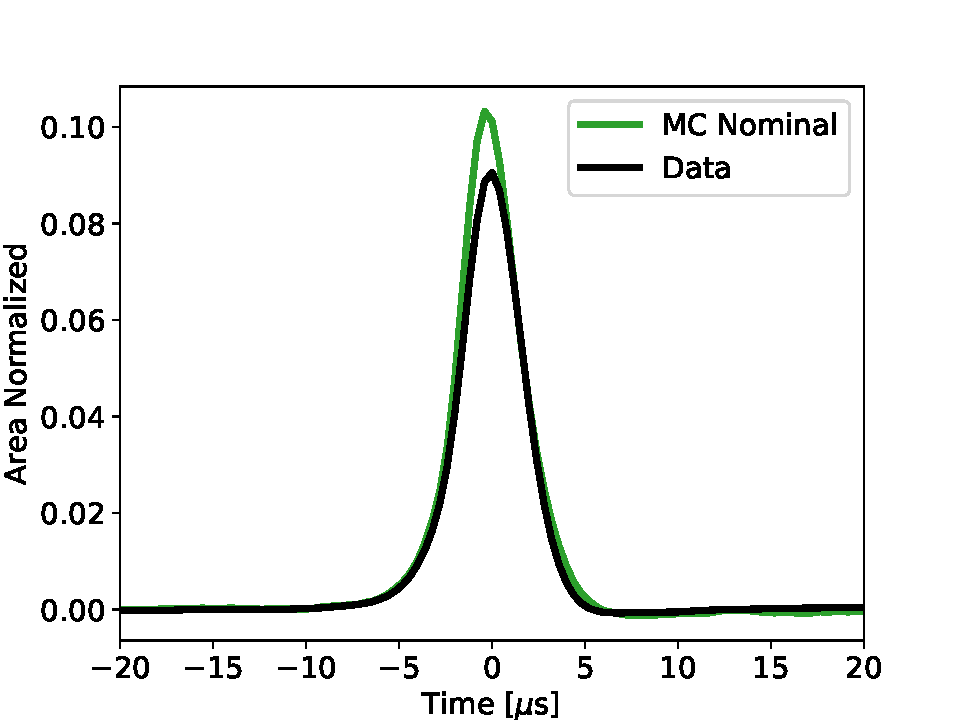
\includegraphics[width=0.3\linewidth]{detector/wvf_data_MCNominal_a20_P2.pdf}\label{fig:TPC_wire_c}}
    \caption[TPC plane signal]{Typical \emph{raw} signal captured by the three planes (induction-1 \ref{sub@fig:TPC_wire_i1}, induction-2 \ref{sub@fig:TPC_wire_i2} and collection \ref{sub@fig:TPC_wire_c}) showing the characteristic bipolar signal for the two induction plane and the unipolar shape for the collection plane. Taken from \cite{ICARUS:2024hmk}. }
    \label{fig:TPC_signal}
\end{figure}

In order to obtain a simplified representation of the information collected by the wireplanes, three major steps are addressed in \emph{Stage0}: \begin{inparaenum}
    \item the wire signals are deconvolved from the TPC electronic response functions, so that all three wire signal are also unipolar in shape;
    \item the signal is analysed in order to define the region-of-interest (ROI) with a threshold-based algorithm; 
    \item each ROI is finally fit using a Gaussian function, whose area is proportional to the number of drift electrons generating the signal. 
\end{inparaenum}

\paragraph{Wire signal processing} The raw decoded wire signal shape is dependent on the distribution of drift electrons, which is core to obtaining calorimetric and particle identification information, but in order to explain such dependency, the raw signal must be processed. The resulting signal $R(t)$ on the wires can be seen as the convolution of serial effects of signal formation, electron propagation, electrostatic field response around the wires and processing by the DAQ to the true electronic signal, so that the response function can be factorised as \begin{equation}
    \begin{aligned}
        R(t, t')&=\mathrm{Ionization\ \otimes\ Recombination\ \otimes\ Diffusion\ and\ Attachment\ \otimes} \\
        &\quad \quad \mathrm{\otimes\ Field\ response\ \otimes\ Electronic\ response\ \otimes\ Electronic\ noise}
    \end{aligned} 
\end{equation} In order to recover the desired ionisation electron yield, useful to have a knowledge of the deposited energy per wire inside the detector as a function of time, it is necessary to unfold these effects. 

The ICARUS detector exploit a signal processing chain similar to other LArTPC experiments, performing a deconvolution in time of the signal waveforms. Ideally, after the deconvolution step, the signal pulse produced by a charged track on the wire would be Gaussian-shaped, with an integral area proportional to the deposited energy inside LAr. The signal recorded on the wires is the convolution of the response function $R$ with the ``true'' $S$ signal, \begin{equation}
    M(t') = \int_{-\infty}^{+\infty} R(t'-t)\ S(t)\ \dd t;
\end{equation} Using the properties of the Fourier transforms, this can be written in the frequency space as $\mathcal M(\omega) = \mathcal R(\omega)\cdot \mathcal S(\omega)$, which can be easily inverted, retrieving the ``true'' signal shape $\mathcal S(\omega)$. This approach, referred to as ``one-dimensional'' deconvolution, is currently employed in most of LArTPC detectors. However, this assumes that the charge distribution on each wire is independent on the charge distribution on the wires in its vicinity. It has been demonstrated that this is not completely true, as can be seen in references \cite{MicroBooNE:2018swd,MicroBooNE:2018vro}. Though it implies small corrections to the overall deposited charge in general, this is not always the case. For example, for isochronous tracks (i.e. tracks lying parallel to the wires, which is somewhat common for the induction-1 wires given the ICARUS geometry), these vicinity effects can create destructive interference patterns.

\begin{figure}
    \centering
    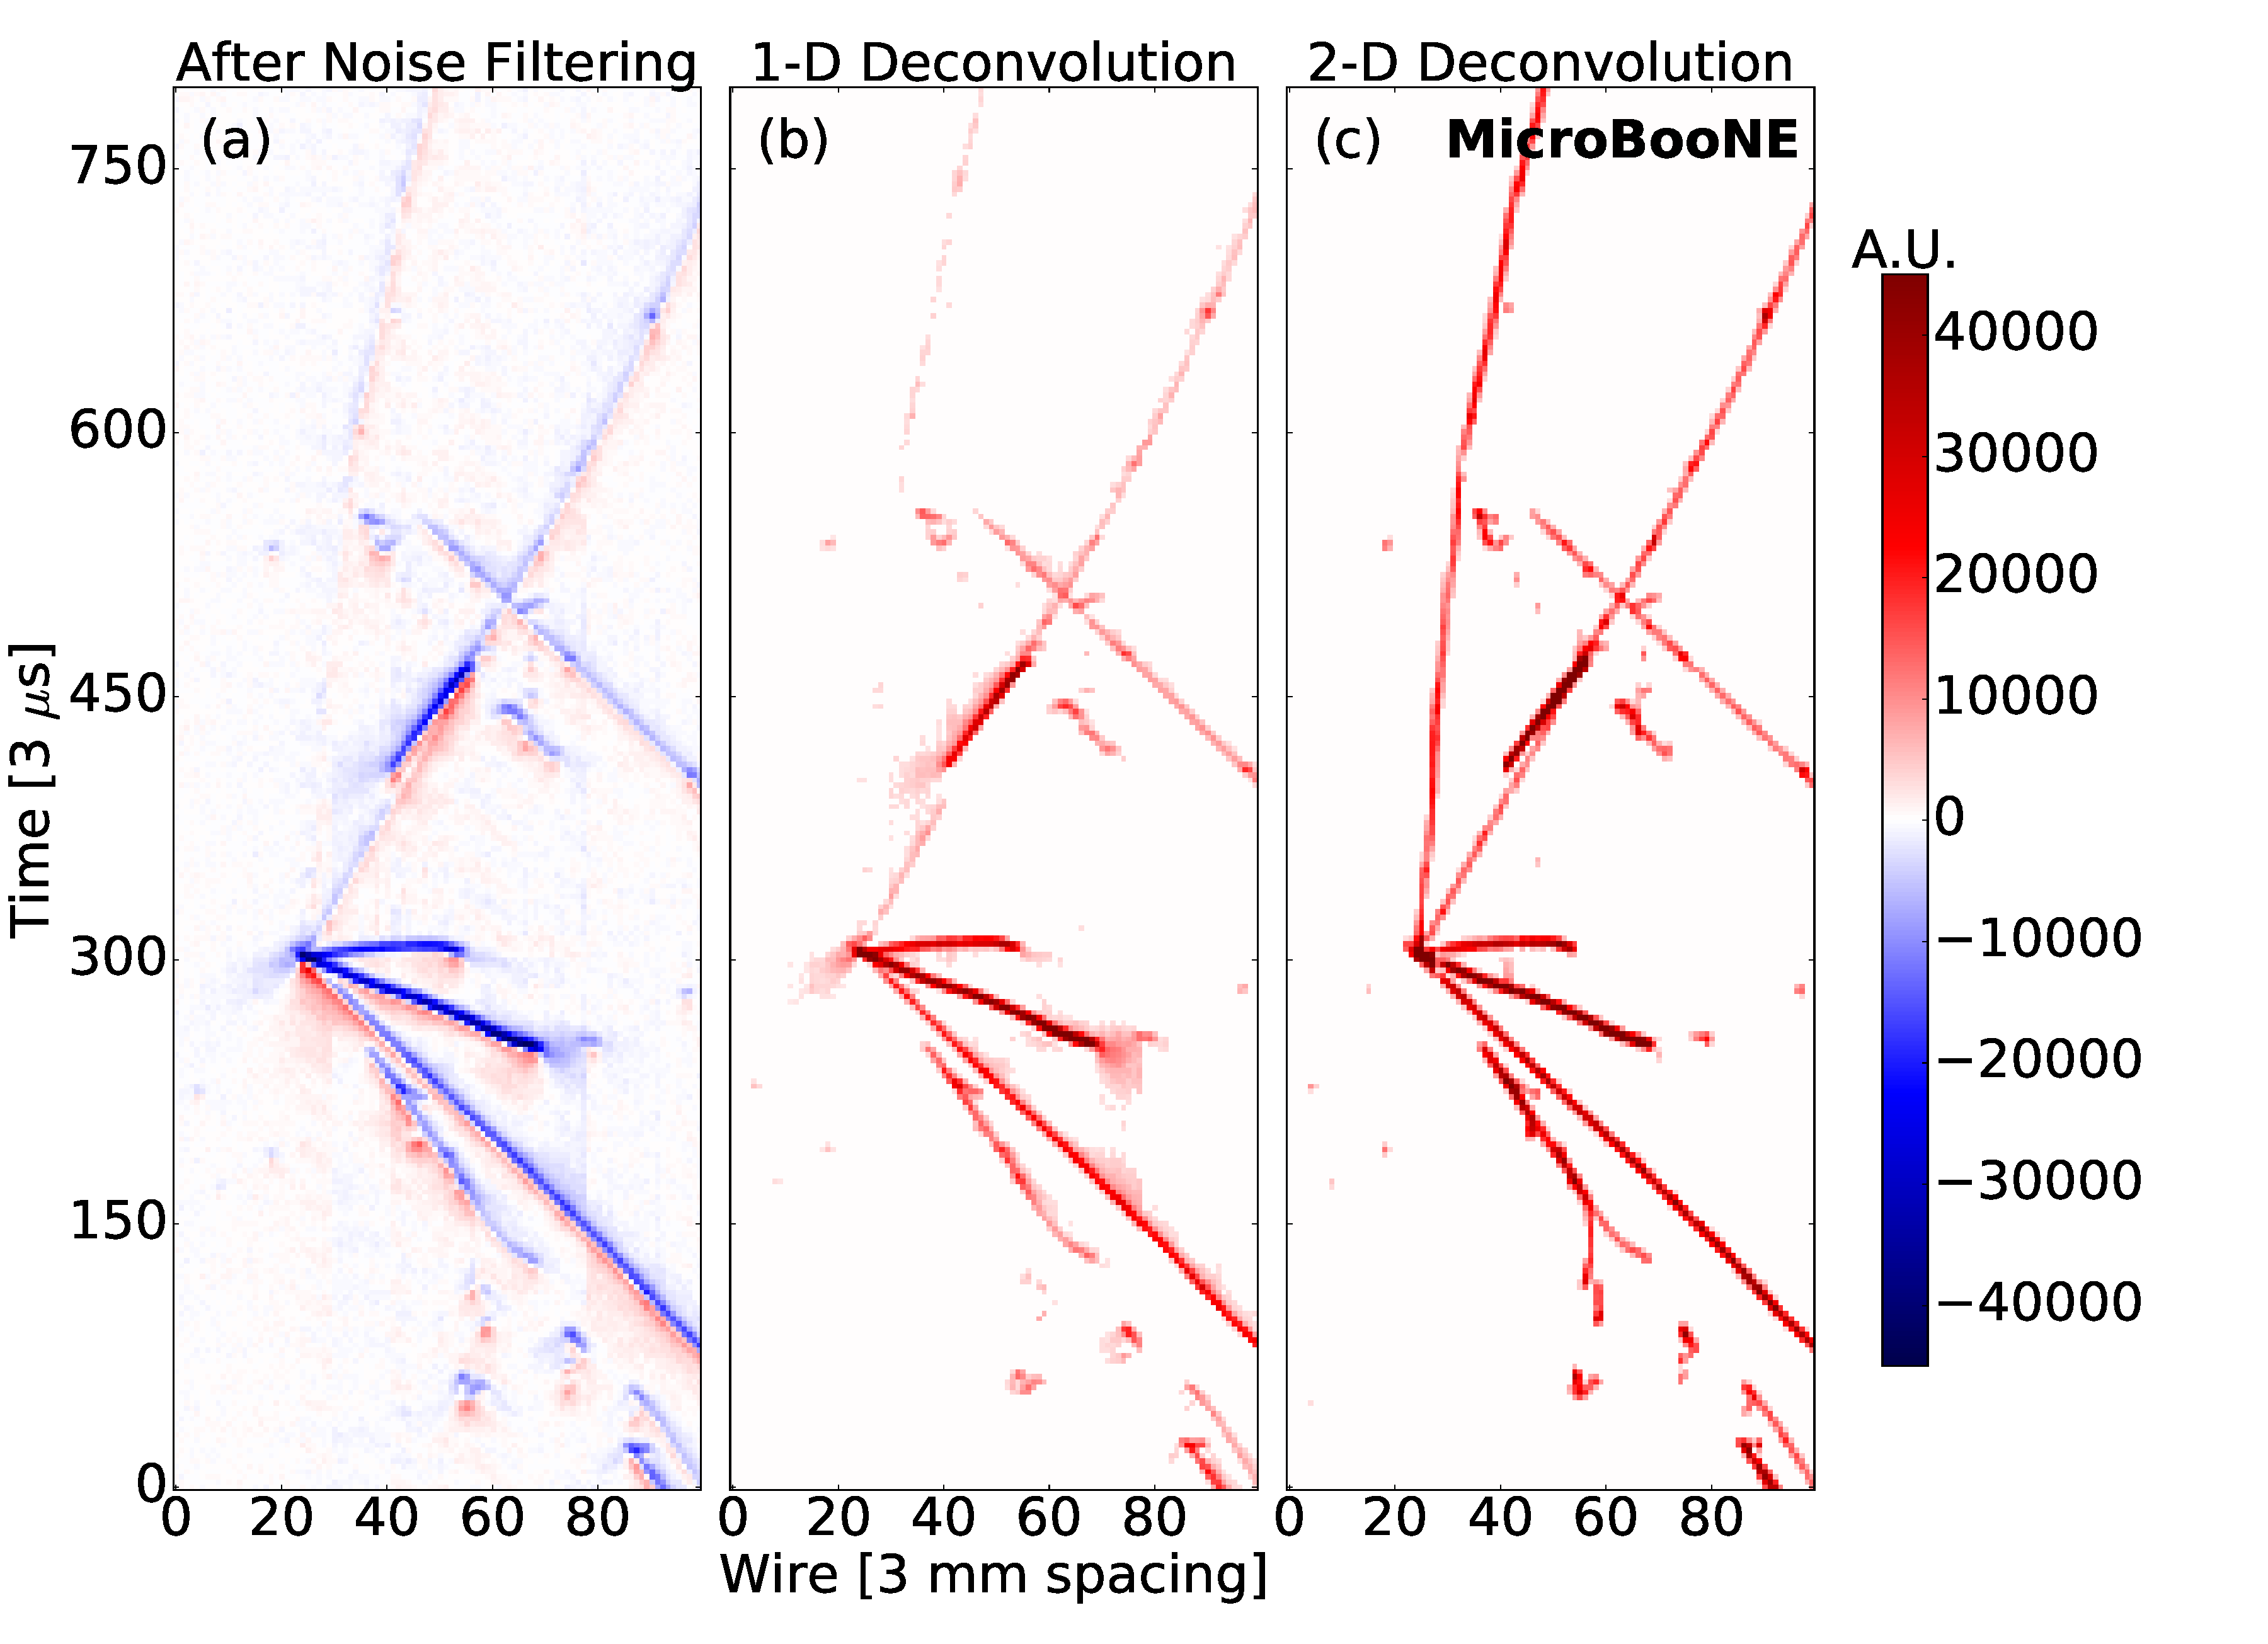
\includegraphics[width=0.85\linewidth]{detector/noiseVs1DVs2D.pdf}
    \caption[TPC signal processing]{Example of the effect of signal processing using the one-dimensional deconvolution approach used in ICARUS (b) with respect to the noise-filtered data (a). (c) shows the same event using a two-dimensional deconvolution approach, performing the deconvolution both in the time direction as well as in the direction of the wires. Taken from \cite{MicroBooNE:2018swd}. }
    \label{fig:uBooNE_signalProc}
\end{figure}

In \cite{MicroBooNE:2018swd,MicroBooNE:2018vro} a solution, adopting two-dimensional deconvolution techniques over both the wire time as well as the wire number, is presented; these provide a strong and computationally efficient method to better extract the distribution of ionisation electrons. \autoref{fig:uBooNE_signalProc} shows the result of the 1D and 2D approaches as tested by the MicroBooNE detector. Tests towards adapting the 2D signal deconvolution are being made, and once validated, should provide a better reconstruction efficiency for the ICARUS TPC detector. 

\paragraph{ROI finding} Once the signal is unipolar in all planes, the next step to define the TPC hits is to select only the ``interesting'' regions of the wires. These regions of interest (ROI) are identified by performing a threshold search in the time domain, allowing to restrict the area on which the \emph{Hits} are created to small portions of the wires. ROIs can be actually relevant to iteratively improve the performances of the 1D/2D deconvolution steps, minimising the time-domain region over which the deconvolution is performed. Once ROIs are identified, a baseline value can be assumed for all other times in the waveform, drastically reducing the size of these data products inside the data files. 

\paragraph{\emph{Hit} creation} Upon the identification of ROIs, the final step is the creation of the \emph{Hit}s objects. A \emph{Hit} is a two-dimensional object representing a cluster of electric drift charges, arriving at a certain time on a certain wire. The \emph{Hit} finding algorithm runs under the assumption the distribution of the drift charges is gaussian. Operating on the deconvolved ROI segments of the waveforms, it tries to fit one or multile Gaussian distributions onto the signal shape. The extracted parameters from the fit process of the Gaussian distribution(s) --- the area, FWHM, the mean, and their multiplicity --- are the properties of the \emph{Hit} objects. The area is proportional to the cumulative charge deposited by the electrons, proportional to the deposited energy inside the detector; the mean and the FWHM represent the \emph{Hit} peak time and its width; the multiplicity can be used to perform operations between adjacent hits. 

At this point, a collection of 2D \emph{Hit}s for each plane of wires has been created. The three 2D views of the planes are stored and used as input for the event reconstruction taking place inside \emph{Stage1}. 

\section{Cosmic ray tagger reconstruction} 

\begin{figure}
    \centering
    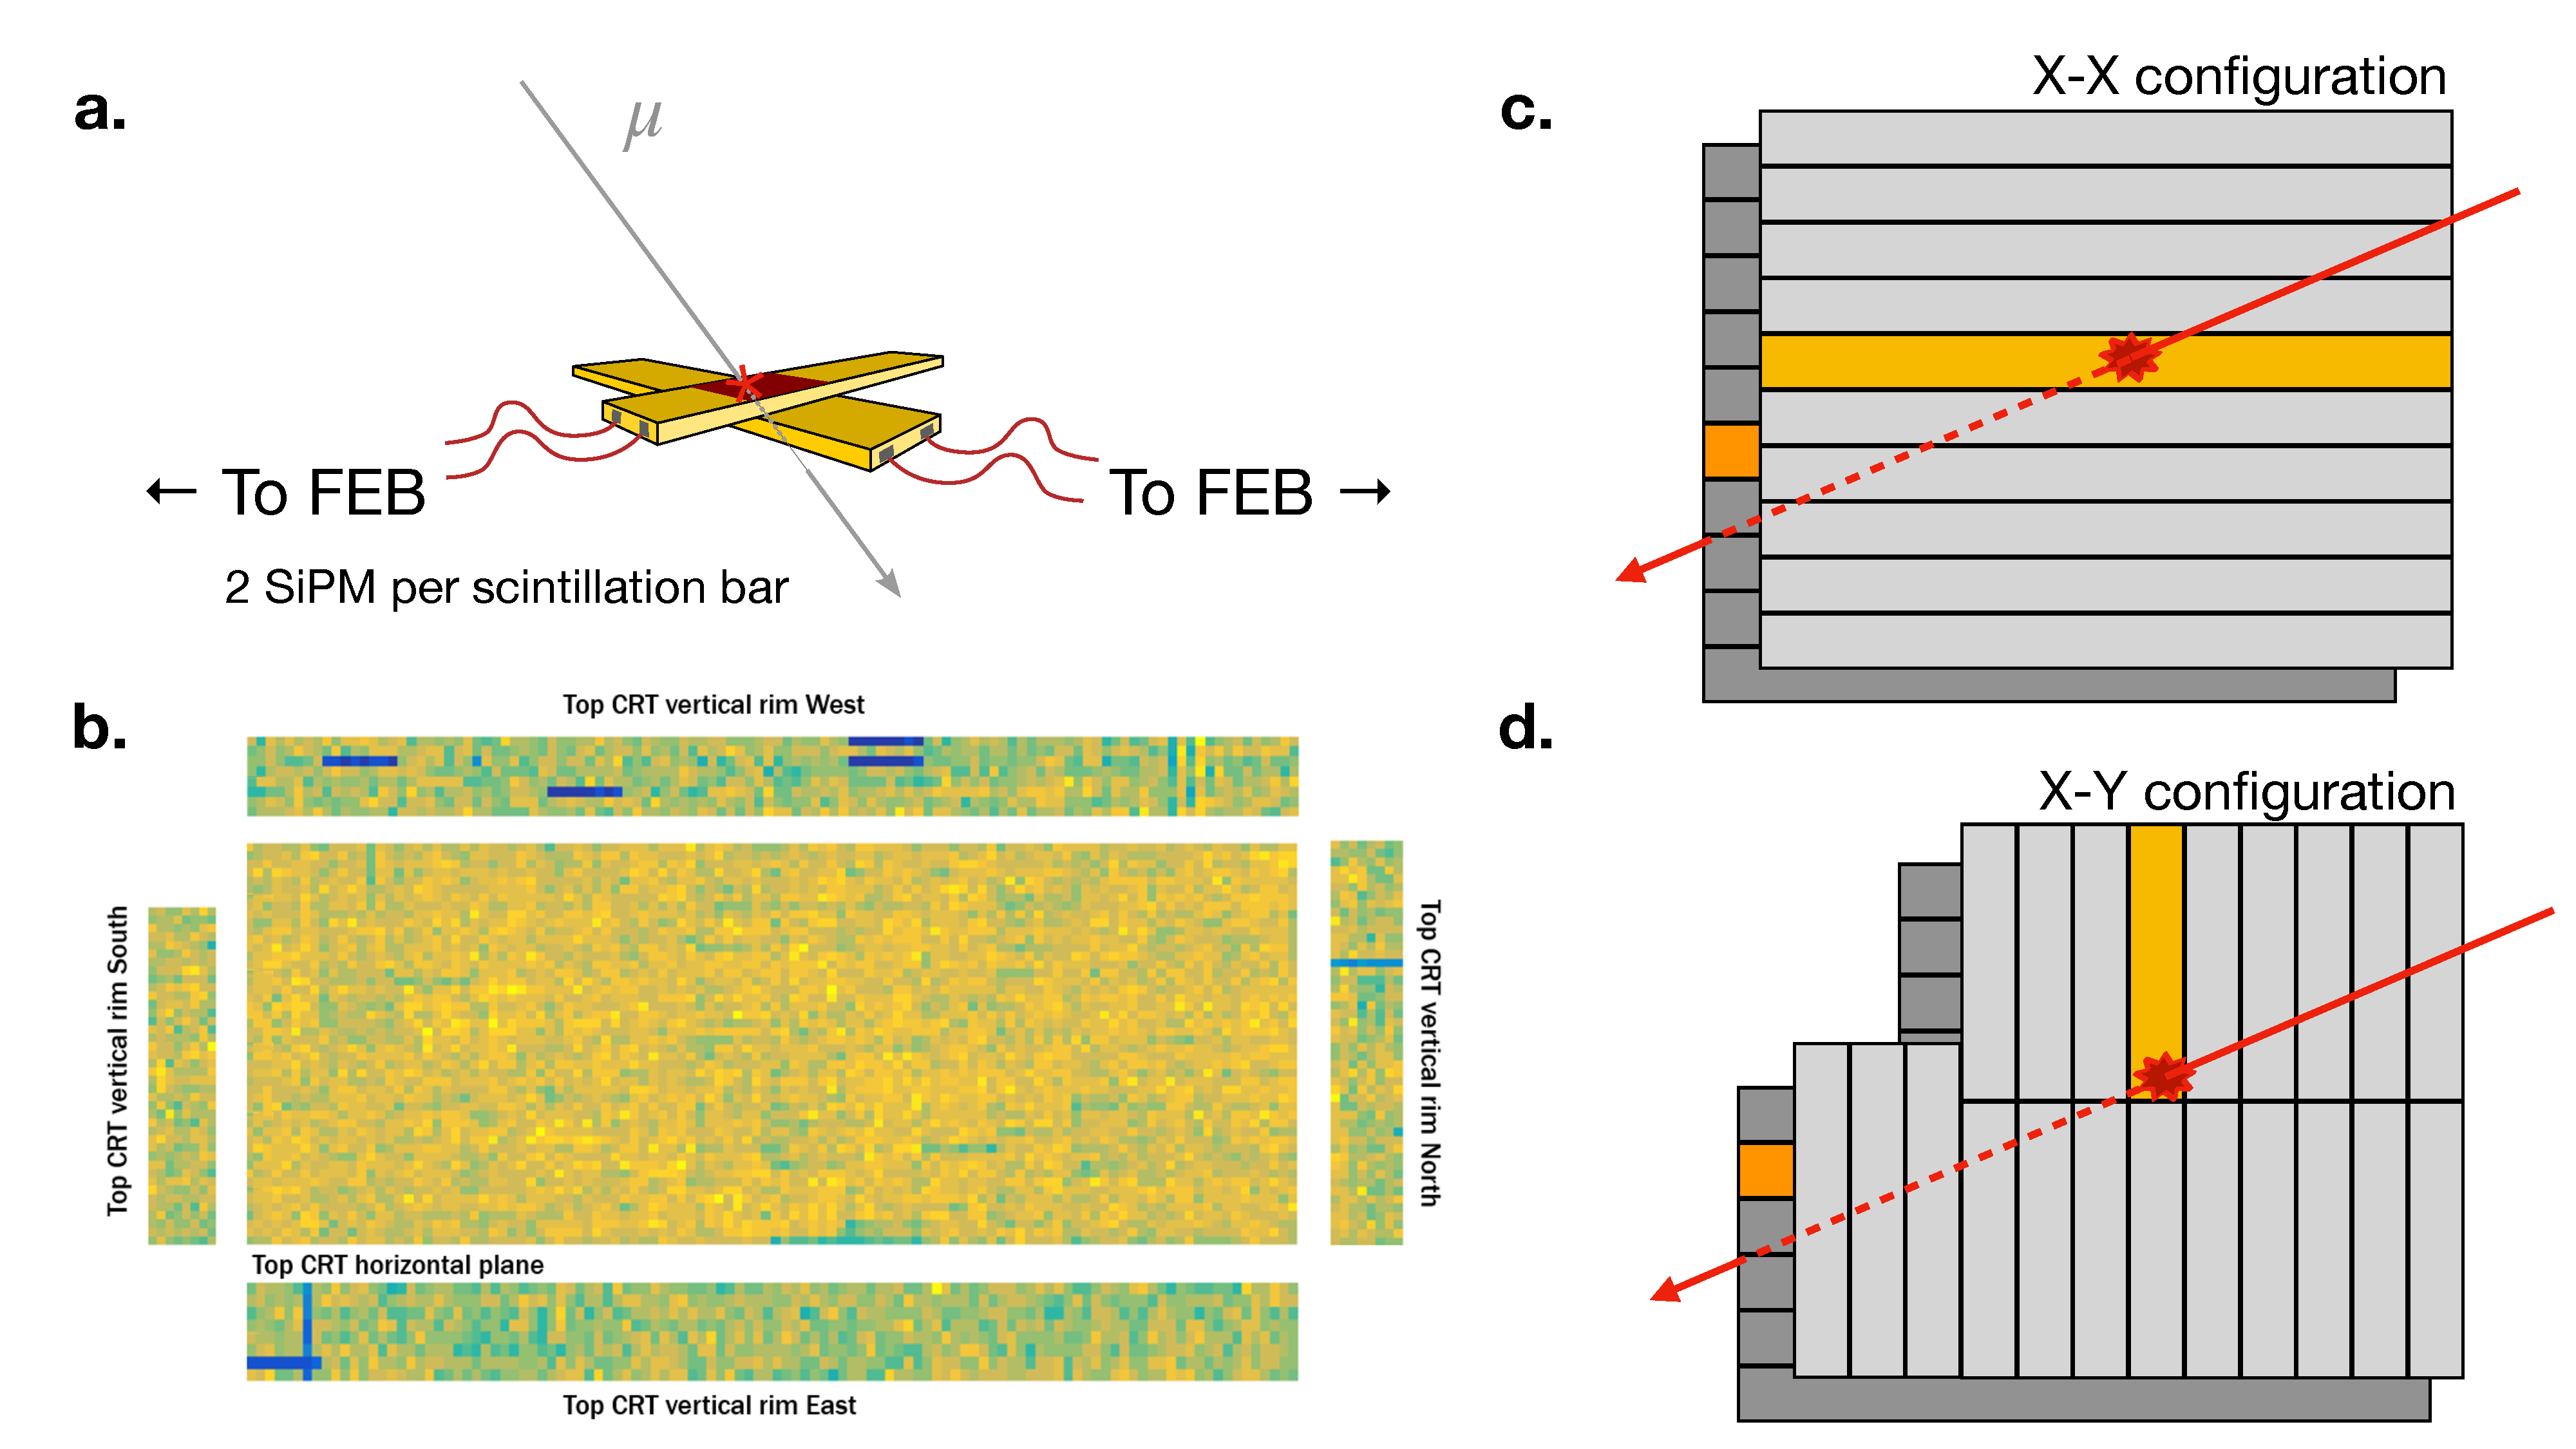
\includegraphics[width=\linewidth]{detector/CRT_all.pdf}
    \caption[CRT Hit reconstruction in space]{Illustration of CRT \emph{Hit} reconstruction position. (a) shows the reconstruction for the top CRT modules, where the coincidence between two scintillation bars is required. (b) shows the distribution of the CRT hits reconstructed in the different regions of the Top CRT. Blue regions
correspond to malfunctioning channels. (b) is taken from \cite{Poppi:2023zmp}, (a), (c) and (d) are adapted from \cite{arteroponsStudyReconstructionNuMuCC}.}
    \label{fig:CRT_reco}
\end{figure}

% \section{TPC event reconstruction}


% \subsection{Sequential approach: Pandora}

% \subsection{Machine Learning approach: SPINE}

%       "crthit",
%       "crttrack",
%       "crtpmt"
%    ]


%  reco: [
%       "cluster3DCryoE",
%       "pandoraGausCryoE",
%       "pandoraTrackGausCryoE",
%       "pandoraKalmanTrackGausCryoE",
%       "SBNShowerGausCryoE",
%       "cluster3DCryoW",
%       "pandoraGausCryoW",
%       "pandoraTrackGausCryoW",
%       "pandoraKalmanTrackGausCryoW",
%       "SBNShowerGausCryoW",
%       "fmatchCryoE",
%       "fmatchCryoW",
%       "fmatchopCryoE",
%       "fmatchopCryoW",
%       "tpcpmtbarycentermatchCryoE",
%       "tpcpmtbarycentermatchCryoW",
%       "caloskimCalorimetryCryoE",
%       "caloskimCalorimetryCryoW",
%       "mcassociationsGausCryoE",
%       "mcassociationsGausCryoW"
%    ]